\documentclass[tikz,border=8pt]{standalone}
% Shared look for every TikZ diagram. Load with \input{../../tools/tikz-style.tex}
\usepackage[T1]{fontenc}
\usepackage{lmodern}
\renewcommand{\sfdefault}{lmr}  % diagrams use the same serif as the text
\usetikzlibrary{arrows.meta, positioning, shapes.geometric, calc, fit, backgrounds}
\definecolor{cblue}{HTML}{4C78A8}
\definecolor{corange}{HTML}{F58518}
\definecolor{cgreen}{HTML}{54A24B}
\definecolor{cred}{HTML}{E45756}
\definecolor{cpurple}{HTML}{B279A2}
\definecolor{cgrey}{HTML}{6B6B6B}
\tikzset{
  every picture/.style={font=\sffamily, line width=1.2pt},
  box/.style={draw=#1, fill=#1!12, rounded corners=4pt, align=center, inner sep=7pt, minimum height=1.1cm},
  box/.default=cgrey,
  arrow/.style={-{Stealth[length=3mm]}, draw=cgrey, line width=1.4pt},
  title/.style={font=\sffamily\bfseries\Large},
  note/.style={font=\sffamily\small, text=cgrey, align=center},
}
\AtBeginDocument{\hyphenpenalty=10000 \exhyphenpenalty=10000}

\begin{document}
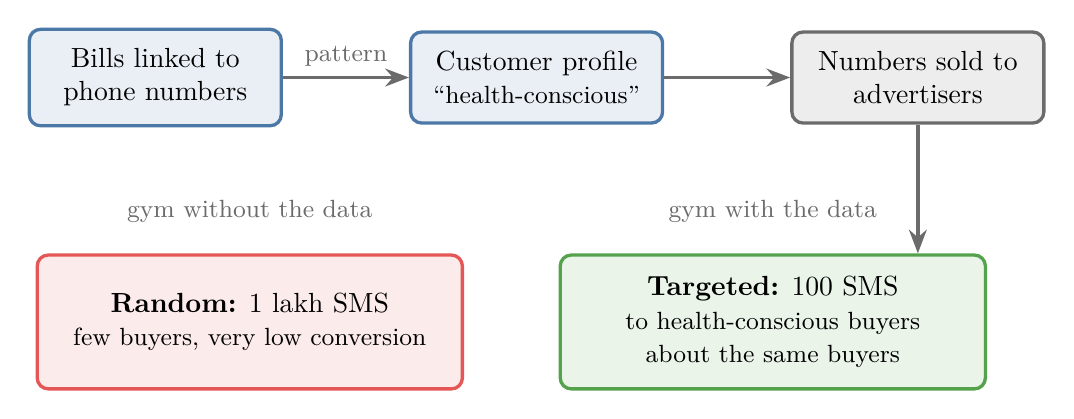
\begin{tikzpicture}[node distance=0.6cm and 1.6cm]
  % top: shop builds profiles
  \node[box=cblue, minimum width=3.2cm] (bill) {Bills linked to\\phone numbers};
  \node[box=cblue, right=of bill, minimum width=3.2cm] (prof) {Customer profile\\{\small ``health-conscious''}};
  \node[box=cgrey, right=of prof, minimum width=3.2cm] (sell) {Numbers sold to\\advertisers};
  \draw[arrow] (bill) -- node[note, above] {pattern} (prof);
  \draw[arrow] (prof) -- (sell);
  % bottom: random vs targeted
  \node[box=cred, below=1.6cm of bill, xshift=1.2cm, minimum width=5.4cm, minimum height=1.7cm] (rand) {\textbf{Random:} 1 lakh SMS\\{\small few buyers, very low conversion}};
  \node[box=cgreen, right=1.2cm of rand, minimum width=5.4cm, minimum height=1.7cm] (targ) {\textbf{Targeted:} 100 SMS\\{\small to health-conscious buyers}\\{\small about the same buyers}};
  \node[note, above=0.25cm of rand] {gym without the data};
  \node[note, above=0.25cm of targ] {gym with the data};
  \draw[arrow] (sell.south) -- (targ.north -| sell.south);
\end{tikzpicture}
\end{document}
